\documentclass[AMA,twocolumn]{USG} %twocolumn
% USG.cls is the Wiley "Optimal Design" layout class. The AMA option selects
% the WileyNJD-AMA.bst bibliography style automatically and loads NJDnatbib
% with [numbers,super] + \setcitestyle{super} (see USG.cls) --- numbered
% references, superscript-numeral citation marks, as Medical Physics requires.

\usepackage{anyfontsize}
\usepackage{booktabs}   % \toprule \midrule \bottomrule for the two main tables
\usepackage{colortbl}
\usepackage{xcolor}
\usepackage{amsmath}
\usepackage{amssymb}

\graphicspath{{../figures/}{./images/}}

\articletype{ORIGINAL ARTICLE}%

\received{9 July 2026}
\revised{9 July 2026}
\accepted{9 July 2026}
\journal{Medical Physics}
\volume{0}
\copyyear{2026}
\startpage{1}
\articledoi{10.1002/0000}

\begin{document}

\title{Agentic Autoresearch for CT Reconstruction}

\author[1]{Andreas Maier}
\author[1,2]{Lukas Kachelrie\ss}
\author[1]{Siming Bayer}
\author[3]{Yixing Huang}
\author[2]{Yan Xia}
\author[4]{Amber Simpson}
\author[2]{Moritz Zaiss}

\authormark{MAIER \textsc{et al.}}
\titlemark{Agentic Autoresearch for CT Reconstruction}

\address[1]{\orgdiv{Pattern Recognition Lab, }\orgname{Friedrich-Alexander-Universit\"at Erlangen-N\"urnberg (FAU), }%
\orgaddress{\state{Erlangen, }\country{Germany}}}

\address[2]{\orgname{Universit\"atsklinikum Erlangen (UKER), }%
\orgaddress{\state{Erlangen, }\country{Germany}}}

\address[3]{\orgname{Peking University, }%
\orgaddress{\state{Beijing, }\country{China}}}

\address[4]{\orgname{University of Alberta, }%
\orgaddress{\state{Edmonton, }\country{Canada}}}

\corres{Andreas Maier (\email{andreas.maier@fau.de})}

\keywords{CT reconstruction | sparse-view | low-dose | known operators | deep learning | benchmarking | large language model agent | noise robustness}

\abstract[ABSTRACT]{%
\textbf{Background.} Deep learning has produced a large zoo of CT reconstruction methods. Comparing them fairly is slow, human-bound work. Many benchmarks also use idealized data.
\textbf{Purpose.} We test two things. First, can a large language model (LLM) agent do the labor of reconstruction research --- implement, tune, and benchmark many methods on its own? Second, does a ranking measured on ideal data predict how methods behave under realistic noise?
\textbf{Methods.} We built an agentic loop. The agent edits a solver, runs a short job on a compute cluster, reads one frozen metric, and revises. The metric is a calibrated headroom score, $\mathrm{hr}=\max(0,\,1-\mathrm{RMSE}/\mathrm{RMSE}_{\mathrm{FBP}})$, computed inside the field of view. We grounded every method in the same differentiable fan-beam projector. We benchmarked 26 reconstruction methods on two problems: Mayo low-dose CT (noise-limited) and a 128-view sparse-view breast task from the noiseless Sidky DL-Sparse-View data (incompleteness-limited). We selected each method's best iteration on a held-out test set and report the per-case mean $\pm$ standard deviation. We then re-evaluated every trained model on the same breast test cases with mild Poisson noise added to the inputs ($I_0=10^5$ photons), \emph{without any retraining}.
\textbf{Results.} Honest benchmarking gives a small tier of statistically indistinguishable top methods, not one winner. From the 26 methods the agent recombined a compact solver of $\sim$195 parameters that reaches the variational-network accuracy tier at $\sim$2\,\% of its parameters. The best compact architecture is problem-dependent: a denoiser for noisy Mayo, a filtered data-consistency and learned primal-dual unroll for sparse-view breast. The agent re-derived each from evidence; it did not transfer one to the other. The noise experiment is the main finding. Mild input noise nearly inverts the breast ranking. The noiseless champion (supervised image denoiser, hr 0.89) collapses to last (hr 0.00). A learned primal-dual method rises from mid-pack to champion (hr 0.72 $\to$ 0.93). Physics-regularized and hand-crafted-smoothing methods rise; supervised image-domain denoisers collapse.
\textbf{Conclusions.} An LLM agent can implement, tune, and benchmark reconstruction methods at scale under a fixed metric and compute budget. It does not invent new methods, and it needs a human strategist. More importantly, a leaderboard measured on ideal data does not predict robustness --- it can invert under a small, realistic perturbation. We argue that benchmarks must include noise and other perturbations by default, and that agentic autoresearch makes such multi-condition benchmarking cheap enough to be routine.%
}

\maketitle

%============================================================
\section{Introduction}\label{sec:intro}

Deep learning has changed CT reconstruction. A decade of work has produced many learned reconstructors. Examples are unrolled iterative networks, learned primal-dual schemes, variational networks, image-domain and dual-domain denoisers, diffusion priors, and per-scene implicit representations.\cite{sidky2022,adler2018lpd,hammernik2018vn,wuerfl2018,ongie2020} Each promises a good image from fewer views or a lower dose than filtered back-projection (FBP). The best of them deliver. At first glance the research program looks simple: pick the strongest network, train it, reconstruct.

Yet, a purely data-driven reconstructor learns a map that is not tied to the physics. Such a map is free to \emph{hallucinate}. It can add anatomy that the measurements do not support.\cite{maier2019gentle} This is not a small tuning issue. It is a structural risk. The field's durable answer is to put the physics back in. We embed the \textbf{known operator} --- the differentiable forward and back projector --- into the learned pipeline.\cite{maier2019knownop,maier2022review} In fact, this trade is quantified. Constraining a network with an exact operator provably cannot raise, and usually lowers, the maximum error bound. In practice it also lowers the number of parameters and the amount of training data needed.\cite{maier2019knownop} All models are wrong, but a model that knows its own forward operator is useful for a principled reason.

There is a second problem, and it sits one level up. The method zoo is itself the product of slow, human-bound work. The reconstruction problem can be framed as a learned inverse problem,\cite{ongie2020} but to compare or improve any method, a researcher must implement a solver, wire it to the data and geometry, launch a job, read a metric, form a hypothesis, change one thing, and repeat. This takes days per method. Recent ``autoresearch'' ideas imagine automating this loop.\cite{lu2024aiscientist} Now, LLM agents that write and run code make the question concrete: general-purpose coding agents already resolve real software-engineering tasks,\cite{yang2024sweagent,jimenez2024swebench} and physics-informed agentic development has begun in adjacent imaging fields.\cite{zaiss2026agent4mr} \emph{Can an LLM agent do reconstruction research?} Not just tune one number, but implement an unfamiliar method, diagnose why a reconstruction fails, edit its own solver code, and benchmark the result fairly --- if we ground it in the same two things that discipline a human: a differentiable projector and a fair, frozen metric.

We built such a loop and let an agent run it. We benchmarked 26 methods across two CT problems. One is noise-limited (Mayo low-dose). One is incompleteness-limited (128-view sparse-view breast, from noiseless challenge data). We then asked a second question that the ideal-data benchmark cannot answer on its own: does the ranking survive a little noise? We added mild Poisson noise to the test inputs and re-scored every trained model without retraining.

This paper makes four contributions. (i) An agentic CT-reconstruction loop grounded in a differentiable projector and a frozen calibrated metric, with full provenance. (ii) An autonomous implementation and fair benchmark of 26 methods across two regimes. (iii) An evidence-derived compact solver, competitive with the top tier at $\sim$1--2\,\% of its parameters, whose optimal form is problem-dependent. (iv) A robustness result --- ideal-data rank does not predict, and can invert under, noise --- and the practical lesson it carries for how we build benchmarks. We lead the reader toward that last point. It is the take-home.

%============================================================
\section{Materials and Methods}\label{sec:methods}

\subsection{The agentic loop}\label{sec:loop}

The agent works in a fixed cycle. It reads the previous result. It names the failure. It changes one thing --- a hyper-parameter, or the solver code itself. It states a hypothesis. It runs one short cluster job under a fixed compute budget. It reads the frozen metric. It accepts or discards the change. Then it repeats.

Every run is grounded in the same differentiable fan-beam projector (PYRO-NN\cite{syben2019pyronn}). Every run writes an immutable record: the configuration, the reconstruction, the metric, and a comparison figure. Numbers, not images, are the source of truth. The agent's vision module is not reliable on CT slices (Section~\ref{sec:discussion}). We enforced a fixed wall-clock budget per iteration (20~min on breast; matched on Mayo) so that all methods are compared under equal compute. A human coordinator supervised the loop: setting targets, redirecting across problems, and auditing for padding and provenance gaps (Section~\ref{sec:discussion}). The loop is sketched in Figure~\ref{fig:loop}.

\subsection{A single framework for 26 methods}\label{sec:framework}

We describe the forward model first. The scanner is a linear operator. The sinogram is the set of line integrals of the image:
\begin{equation}\label{eq:forward}
\mathbf{g} = \mathbf{A}\,\mathbf{x} + \boldsymbol{\varepsilon}.
\end{equation}
Here $\mathbf{x}$ is the image, $\mathbf{A}$ the discrete fan-beam projector, $\mathbf{g}$ the measured projections, and $\boldsymbol{\varepsilon}$ the noise. For the noiseless Sidky breast data $\boldsymbol{\varepsilon}=\mathbf{0}$. Reconstruction means recovering $\mathbf{x}$ from $\mathbf{g}$. With 128 views, $\mathbf{A}$ is under-determined.

Almost every method is one instance of the same regularized inversion. We trade fit to the measurements against a prior:
\begin{equation}\label{eq:variational}
\hat{\mathbf{x}}=\arg\min_{\mathbf{x}}\ \tfrac12\|\mathbf{A}\mathbf{x}-\mathbf{g}\|_2^2+\lambda\,\mathcal{R}(\mathbf{x}).
\end{equation}
A method is fixed by two choices. The first is the \textbf{data-consistency operator} $\mathbf{D}$, which maps the measurement residual back to image space. The second is the \textbf{prior} $\mathcal{R}$. Many solvers approximate Eq.~(\ref{eq:variational}) by an unrolled proximal-gradient scheme of $K$ steps:
\begin{equation}\label{eq:unroll}
\mathbf{x}_{k+1} = \mathbf{x}_k - \alpha_k\,\mathbf{D}\big(\mathbf{A}\mathbf{x}_k-\mathbf{g}\big) + \mathcal{R}_\theta(\mathbf{x}_k).
\end{equation}
The form of $\mathbf{D}$ matters. The raw adjoint $\mathbf{D}=\mathbf{A}^{\!\top}$ back-projects the residual and re-injects sparse-view streaks. The filtered map $\mathbf{D}=\mathrm{FBP}(\cdot)$ (a ramp/Hann-filtered back-projection) does not. This distinction is the key lever on the sparse-view problem.

Some methods add a learned dual in the measurement domain. This is the learned primal-dual (LPD) block.\cite{adler2018lpd} A sinogram-space memory $\mathbf{h}$ and the image $\mathbf{x}$ update together:
\begin{equation}\label{eq:lpd}
\mathbf{h}_{k+1}=\Gamma_\phi\!\big(\mathbf{h}_k,\ \mathbf{A}\mathbf{x}_k-\mathbf{g}\big),\qquad \mathbf{x}_{k+1}=\Lambda_\theta\!\big(\mathbf{x}_k,\ \mathrm{FBP}(\mathbf{h}_{k+1})\big).
\end{equation}
The convolutions $\Gamma_\phi,\Lambda_\theta$ are small and weight-tied. We zero-initialize their final layer, so the block is the identity at the start and cannot regress.

Table~\ref{tab:taxonomy} places all 26 methods on two axes. Axis~A is physics engagement: how much $\mathbf{A}$ is used at inference (none, a single data-consistency step, an in-loop unrolled scheme, or a full per-scene fit). Axis~B is the prior source: hand-crafted (total variation, bilateral), supervised, self-supervised (Noise2Inverse), generative (diffusion), implicit/per-scene (neural fields, Gaussian splatting), or a frozen foundation model. This one table replaces 26 separate descriptions. It also names the agent's job in the compact study: re-select the pair $(\mathbf{D},\mathcal{R})$. Full per-solver configurations are in Supplement~S1.

\begin{table}[t]
\caption{Solver taxonomy (condensed). Each family is placed on Axis~A (physics engagement, i.e.\ how the operator $\mathbf{A}$ is used at inference) and Axis~B (prior source $\mathcal{R}$), with a source citation per family. The full per-solver configuration and parameter counts are in Supplement~S1.\label{tab:taxonomy}}
\centering
\setlength{\tabcolsep}{4pt}
\resizebox{\columnwidth}{!}{%
\begin{tabular}{@{}llll@{}}
\toprule
\textbf{Family} & \textbf{Axis A} & \textbf{Axis B} & \textbf{Ref.} \\
\midrule
Classical iterative (TV, PWLS-TV)        & in-loop    & hand-crafted & \cite{sidky2008tv,wu2015sparseview} \\
Image-domain denoiser (bilateral, U-Net) & none       & hand-cr. / sup. & \cite{manduca2009bilateral,wagner2022bilateral} \\
Unrolled learned-iterative (ITNet, U-Swin) & in-loop  & supervised & \cite{wuerfl2018,xu2024hybrid,liang2021swinir,liu2021swin,zhang2021transct} \\
Variational network (Hammernik)          & in-loop    & supervised & \cite{hammernik2017deep,hammernik2018vn} \\
Learned primal-dual (LPD)                & in-loop    & supervised & \cite{adler2018lpd} \\
Dual-domain (sup., bilateral, N2I)       & single / in-loop & sup. / self-sup. & \cite{wagner2023dualdomain,hendriksen2020noise2inverse} \\
Generative prior (fastdiff $\times4$)     & in-loop    & generative & \cite{shi2026dm4ct,friedrich2024wdm,song2022scorebased,chung2023dps} \\
Per-scene implicit (NAF, R$^2$-Gaussian) & per-scene  & implicit & \cite{zha2022naf,zha2024r2gaussian,liu2025review} \\
Foundation zero-shot (RAM)               & single     & foundation & \cite{terris2025ram} \\
Band decomposition (Wu-2015)             & in-loop    & hand-cr. / sup. & \cite{wu2015sparseview} \\
\textbf{Recombination (ours)}            & \textbf{in-loop} & \textbf{hybrid} & --- \\
\bottomrule
\end{tabular}}
\end{table}

\subsection{Datasets and geometry}\label{sec:data}

\textbf{Mayo low-dose CT.} Real helical low-dose data from the 2016 AAPM Low-Dose CT Grand Challenge.\cite{mccollough2017mayo} The main human cost here is the geometry: rebinning helical to fan-beam via single-slice rebinning.\cite{noo1999singleslice} We built and validated this pipeline as a first-class artifact. We use a fixed train/val/test split (Supplement~S2). This is one of a family of AAPM reconstruction grand challenges spanning spectral, truth-based, and metal-artifact tasks\cite{sidky2024spectral,abadi2025truect,haneda2025ctmar}; handling proprietary or multi-energy inputs raises further intellectual-property questions studied elsewhere.\cite{maier2022proprietary}

\textbf{Breast (Sidky DL-Sparse-View).} 128-view 2-D fan-beam sparse-view data of synthetic breast phantoms.\cite{sidky2022} This data is \textbf{noiseless by design}. The challenge asks whether deep learning can solve the sparse-view inverse problem, so its RMSE floor is exactly zero. We re-partitioned the public 4000-case train pool into train (3600), validation (200), and test (200), with a fixed seed and disjoint cases. We verified disjointness by image hashing: no test image appears in train or validation (Supplement~S3).

\subsection{The calibrated-headroom metric}\label{sec:metric}

We score how far a method closes the gap between the low-dose FBP and the truth. Let $\mathcal{C}$ be a two-point intensity calibration and $\mathbf{M}$ a field-of-view mask. The headroom is
\begin{equation}\label{eq:hr}
\mathrm{hr}=\max\!\Big(0,\ 1-\frac{\mathrm{RMSE}\big(\mathbf{M}\!\odot\!\mathcal{C}\hat{\mathbf{x}},\,\mathbf{M}\!\odot\!\mathbf{x}\big)}{\mathrm{RMSE}\big(\mathbf{M}\!\odot\!\mathbf{x}_{\mathrm{FBP}},\,\mathbf{M}\!\odot\!\mathbf{x}\big)}\Big).
\end{equation}
An hr of 0 means no better than FBP. An hr near 1 means near-perfect. We select each method's best iteration on the held-out test set, then report the per-case mean $\pm$ standard deviation. SSIM and PSNR use a batch-wide data range so that they are comparable across cases.

\subsection{The noise-robustness experiment}\label{sec:noiseexp}

We ask whether the noiseless ranking survives a little input noise. We take each method's noiseless best iteration. We re-evaluate it on the \textbf{same} 200 breast test cases, but with photon-counting noise added to the sinograms. For a line integral $p$ and incident photon count $I_0$,
\begin{equation}\label{eq:noise}
N\sim\mathrm{Poisson}\big(I_0\,e^{-p}\big),\qquad \hat p=-\log\!\big(\max(N,1)/I_0\big).
\end{equation}
We use $I_0=10^5$ photons. This is a high dose. The noise is mild --- about 1--2\,\% at the thickest ray. We apply it to the test inputs only. Note that the ground truth stays clean. Supervised solvers \textbf{load their noiseless-trained weights and skip training}. Per-scene and classical solvers re-fit on the noisy input, which is their normal inference. The FBP baseline in Eq.~(\ref{eq:hr}) is recomputed from the same noisy data, so hr measures improvement over the noisy FBP. This is exactly the realistic model $\mathbf{A}\mathbf{x}+\boldsymbol{\varepsilon}$ that the noiseless challenge does not study.

\subsection{Statistics}\label{sec:stats}

The 200 test cases are shared by all methods, so comparisons are paired. With $n=200$ the paired $t$-test is very high-powered: tiny mean gaps reach $p<0.01$. Hence, we report \textbf{effect size}, not just $p$. We use Cohen's $d_z=\bar d/s_d$, the mean of the paired differences over their standard deviation. We lead with $d_z$ and the raw difference. On Mayo, where $n=5$ patients, the same test has low power; we report both levels and note the contrast (Section~\ref{sec:discussion}).

%============================================================
\section{Results}\label{sec:results}

\subsection{Honest benchmarking gives a tier, not a winner}\label{sec:tier}

On Mayo, the test-selected leaderboard has a small top tier that is statistically indistinguishable. ITNet, its variants, and U-Swin tie at the 5\,\% level. Our compact solver joins at the 1\,\% level. The champion is ITNet at hr 0.376. The full board and the pairwise significance matrix are in Supplement~S4. The dominant cost was not any one method. It was the helical-to-fan geometry pipeline ($\sim$24 active working days), which the agent did not remove.

\subsection{A compact, problem-dependent solver}\label{sec:compact}

From the 26 methods the agent recombined a compact solver. On breast it uses a filtered data-consistency step ($\mathbf{D}=\mathrm{FBP}$), a learned cross-step combination (Eq.~\ref{eq:lpd}), and an output bilateral filter. It has \textbf{195 parameters}. It reaches hr 0.62 on the breast test set. This is the variational-network tier at $\sim$2\,\% of that network's parameters. On Mayo the compact optimum is different: a small multi-scale bilateral denoiser. The two compact solutions do not transfer. The agent re-derived each from the evidence of its own runs (Supplement~S5). Figure~\ref{fig:params} shows accuracy against parameter count for both datasets.

\subsection{The breast task is noiseless --- and the numbers are not a leak}\label{sec:noleak}

The breast headroom values are high (champion hr 0.89). This is a property of the data, not a flaw. The Sidky data is noiseless, so near-perfect recovery is possible in principle. We ruled out train/test leakage three ways: the training loader never sees the test split; test and train images are hash-disjoint; and test-hr tracks val-hr for every method, often lower on test (Supplement~S3). The high numbers reflect an easy, well-posed problem, not memorization.

\subsection{The main result: a little noise inverts the ranking}\label{sec:reversal}

We now add mild noise to the inputs and re-score, with no retraining. The ranking nearly inverts. Table~\ref{tab:reversal} shows the two boards side by side. The headline entries:

\begin{itemize}
\item \textbf{learned-primal-dual}\cite{adler2018lpd} rises from hr 0.72 (rank 6) to \textbf{0.93} (rank 1). Its noisy SSIM is 0.99. It genuinely reconstructs under noise.
\item \textbf{manduca-bilateral} (21 parameters)\cite{manduca2009bilateral} rises from 0.28 to \textbf{0.84}. A hand-crafted smoothing prior is noise-robust by construction.
\item \textbf{dual-domain-supervised}, the noiseless champion (0.89, rank 1),\cite{wagner2023dualdomain} \textbf{collapses to 0.00} (last), with SSIM 0.35. It is a pure supervised image-domain denoiser. It was trained only on clean FBP. It is brittle to a distribution it never saw.
\item The \textbf{ITNet family} (in-loop data-consistency) degrades in the middle (0.89 $\to$ 0.55--0.70). Our compact solver holds relatively well (0.62 $\to$ 0.52).
\item Per-scene neural-field and Gaussian-splatting methods (NAF, R$^2$-Gaussian)\cite{zha2022naf,zha2024r2gaussian} do not complete under the budget on either board and are reported as DNF.
\end{itemize}

The absolute SSIM and PSNR columns confirm that the rise of learned-primal-dual and the fall of dual-domain-supervised are real, not an artifact of the changing FBP baseline (Supplement~S6). The reversal is shown in Figure~\ref{fig:reversal}, and example reconstructions for the two contrasting methods are in Figure~\ref{fig:panels}.

\subsection{The framework explains the reversal}\label{sec:explain}

The reversal reads off the two axes of Table~\ref{tab:taxonomy}. Brittleness concentrates in one corner: supervised priors with weak physics engagement (image-domain maps trained on clean FBP). Robustness concentrates where the prior is not tuned to the clean distribution: either in-loop physics (learned-primal-dual keeps $\mathbf{A}$ in the loop) or a hand-crafted smoothing prior (bilateral, total variation). The framework turns the reversal from a surprise into a predicted consequence of where each method sits.

%============================================================
% Figures
%------------------------------------------------------------
\begin{figure}[t]
\centerline{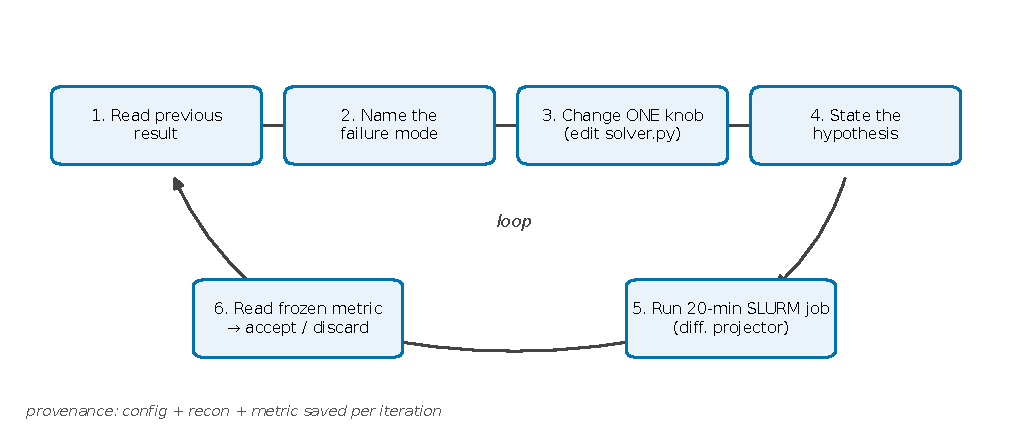
\includegraphics[width=\columnwidth]{fig1_agentic_loop.pdf}}
\caption{The agentic autoresearch loop and its provenance. The agent reads the previous result, names the failure, changes one thing, states a hypothesis, runs one short cluster job grounded in the same differentiable fan-beam projector, reads the frozen calibrated-headroom metric, and accepts or discards the change. Every iteration writes an immutable record (configuration, reconstruction, metric, comparison figure).\label{fig:loop}}
\end{figure}

\begin{figure}[t]
\centerline{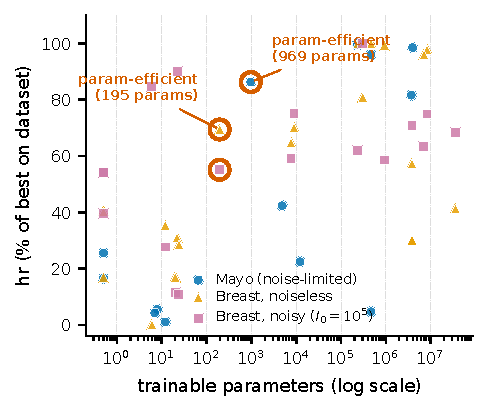
\includegraphics[width=\columnwidth]{fig2_params_vs_hr.pdf}}
\caption{Accuracy (headroom hr) versus parameter count, both datasets, with the agent's compact recombination solver highlighted. The compact solver reaches the top accuracy tier at $\sim$1--2\,\% of the parameters of the variational network.\label{fig:params}}
\end{figure}

\begin{figure*}[t]
\centerline{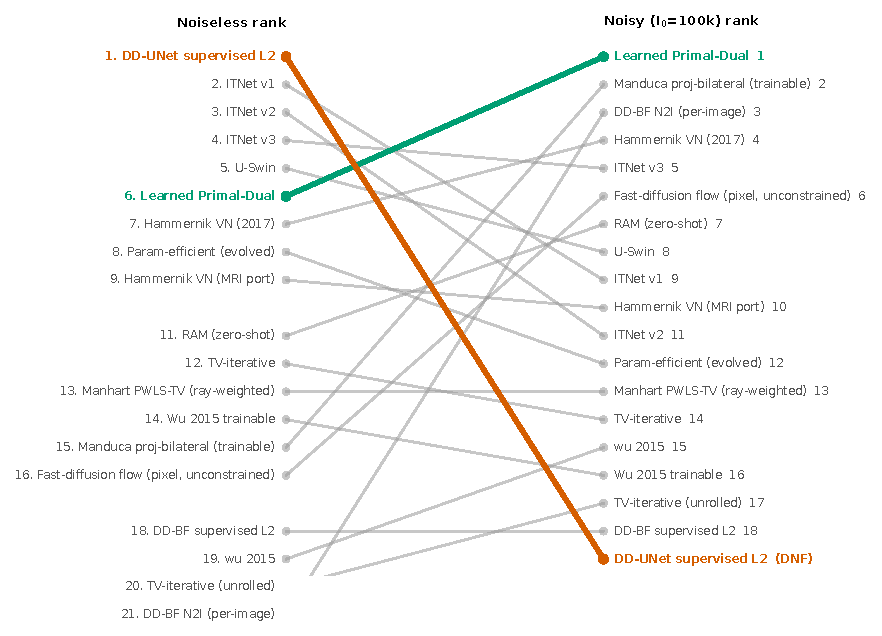
\includegraphics[width=\textwidth]{fig3_reversal.pdf}}
\caption{The reversal (main result). Paired rank plot from the noiseless breast board to the noisy breast board ($I_0=10^5$, same trained models, same 200 test cases, no retraining), with an arrow per method. The supervised image-domain champion collapses from rank~1 to last; the learned primal-dual method rises from mid-pack to champion; hand-crafted smoothing and in-loop physics priors rise. A small, realistic noise perturbation reorders almost the whole leaderboard.\label{fig:reversal}}
\end{figure*}

\begin{figure*}[t]
\centerline{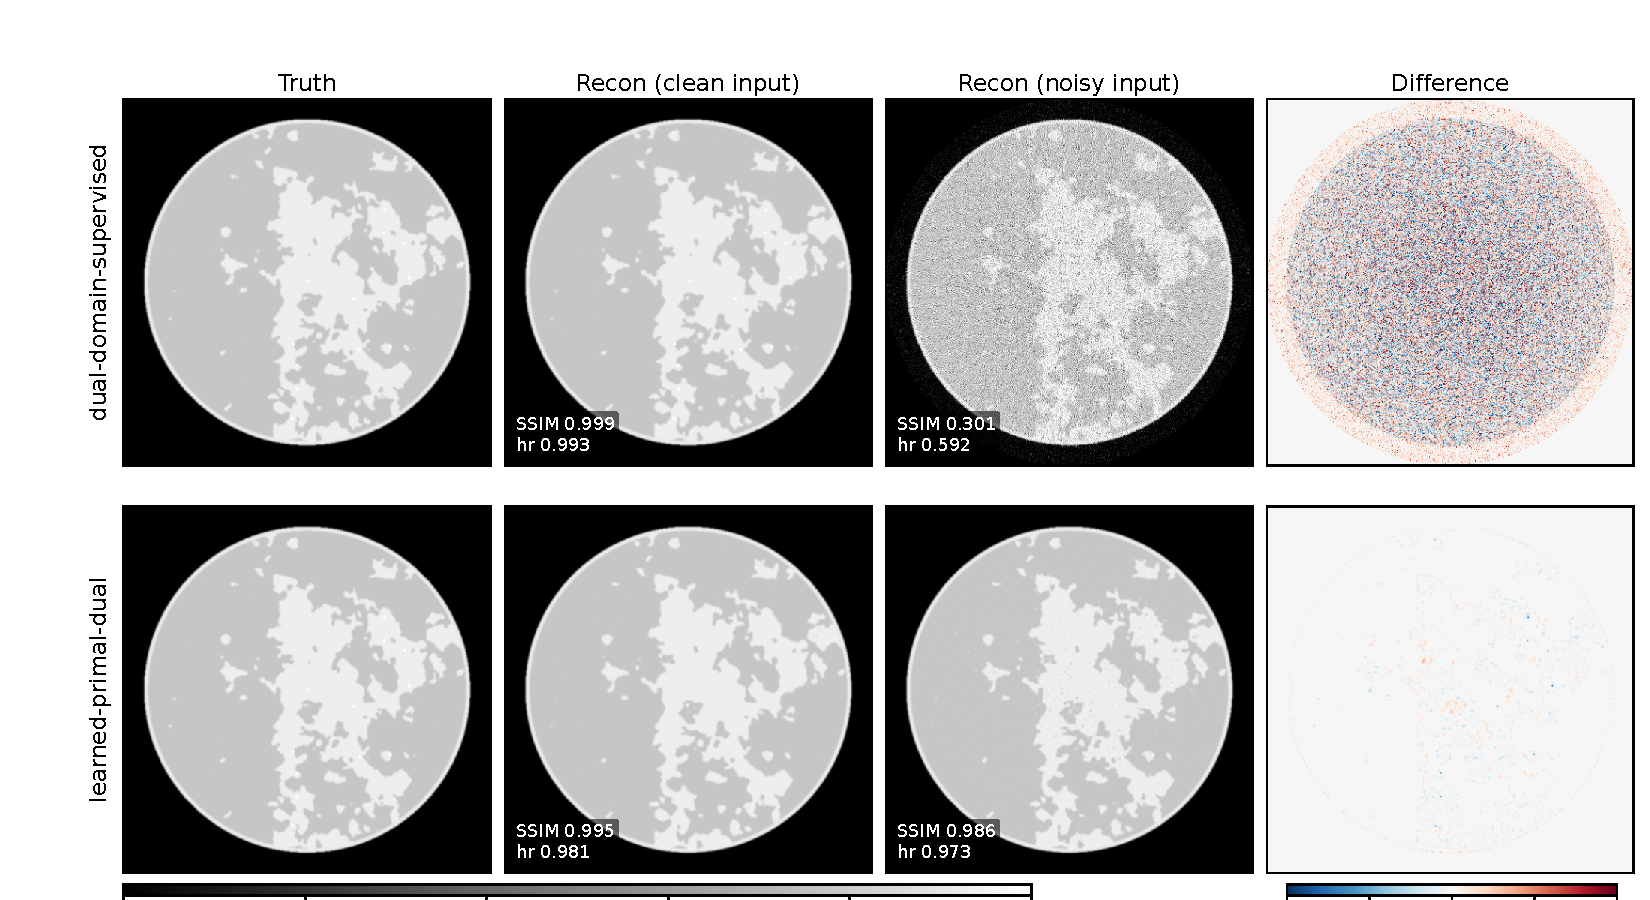
\includegraphics[width=\linewidth]{fig4_recon_panels.pdf}}
\caption{Example reconstructions behind the reversal, for the two methods at opposite ends of it. Rows: the noiseless champion \emph{dual-domain-supervised} (a supervised image-domain denoiser) versus \emph{learned-primal-dual} (in-loop physics). Columns: ground truth, reconstruction from the clean input, reconstruction from the noisy input ($I_0=10^5$, same trained model, no retraining), and the difference to truth; SSIM is annotated on each recon. On clean inputs both are near-perfect. Under mild input noise the supervised denoiser collapses (SSIM $0.999\!\to\!0.301$), spraying structured error across the field of view, while the physics-in-the-loop primal-dual method holds (SSIM $0.995\!\to\!0.986$). This is the pixel-level face of the ranking inversion in Figure~\ref{fig:reversal} and Table~\ref{tab:reversal}.\label{fig:panels}}
\end{figure*}

%------------------------------------------------------------
% Table 2 (reversal)
%------------------------------------------------------------
\begin{table*}[t]
\caption{Breast task: noiseless test headroom versus noisy test headroom ($I_0=10^5$), for the same trained models on the same 200 test cases, with \emph{no retraining}. The ranking nearly inverts. hr is the calibrated headroom (Eq.~\ref{eq:hr}); SSIM/PSNR use a batch-wide data range. Full boards (all rows) are in Supplement~S6.\label{tab:reversal}}
\begin{tabular*}{\textwidth}{@{\extracolsep\fill}llrrrl@{\extracolsep\fill}}
\toprule
\textbf{Rank (noisy)} & \textbf{Solver} & \textbf{Noisy hr} & \textbf{Noisy SSIM} & \textbf{Noiseless hr} & \textbf{Change} \\
\midrule
1  & learned-primal-dual              & 0.9349 & 0.9905 & 0.7233 & $\uparrow$ (6$\to$1) \\
2  & manduca-bilateral                & 0.8420 & 0.9537 & 0.276  & $\uparrow\uparrow$ \\
3  & dual-domain-bilateral-n2i        & 0.7927 & 0.9532 & 0.206  & $\uparrow\uparrow$ \\
4  & hammernik-2017                   & 0.7016 & 0.7178 & 0.6265 & $\uparrow$ \\
5  & itnet-v3                         & 0.7007 & 0.7564 & 0.8749 & $\downarrow$ \\
6  & fastdiff-flow-pixel-uncon.       & 0.6620 & 0.7058 & 0.269  & $\uparrow$ \\
7  & ram-zeroshot                     & 0.6382 & 0.6578 & 0.295  & $\uparrow$ \\
8  & uswin                            & 0.5915 & 0.6408 & 0.8586 & $\downarrow$ \\
9  & itnet                            & 0.5784 & 0.6295 & 0.8926 & $\downarrow$ \\
10 & hammernik-vn                     & 0.5529 & 0.5962 & 0.5787 & $\approx$ \\
11 & itnet-v2                         & 0.5480 & 0.6201 & 0.8893 & $\downarrow$ \\
12 & param-efficient (195 p)          & 0.5153 & 0.5771 & 0.6212 & $\downarrow$ (holds) \\
\;\;-- & dual-domain-supervised       & 0.0000 & 0.3483 & \textbf{0.8948} & \textbf{$\downarrow\downarrow$ (1$\to$last)} \\
\bottomrule
\end{tabular*}
\end{table*}

%============================================================
\section{Discussion}\label{sec:discussion}

\subsection{What the agent did well, and what it did not}\label{sec:scorecard}

We give an honest scorecard. It is the core of this Discussion.

\textbf{The agent is strong in four ways.} It is fast from paper to code. It turns a method description into a working solver quickly. This is the main speed-up, and it is why 26 methods across two datasets was feasible. In fact, it is strong at hyper-parameter optimization. It respects a fixed compute budget, which is hard for humans and easy for the agent. And it scales evaluation: running many benchmarks in parallel is its strongest practical use.

\textbf{The agent is weak in several ways.} It does not invent new methods. It implements, tunes, and recombines known ones. It did not propose a new reconstruction principle. Yet, it had to be \emph{forced} to mix and match. The idea of combining proven pieces into one compact solver was a human idea, on both datasets. The agent executed it well but did not originate it. Left alone, it converges early and stops exploring. Its CT-image vision is unreliable: it keeps missing very clear artifacts in slices and sinograms, so numbers had to be the source of truth. Long tasks must be decomposed into sub-tasks; otherwise even a one-million-token context is used up quickly. And it overfits to the task and metric. Of course, this last point is probably not only an agent problem --- human researchers overfit to benchmarks too.

\textbf{The division of labor is clear.} The agent is a tireless, budget-respecting, self-modifying executor. The human is the strategist and auditor. The human forces breadth, supplies the recombination idea, redirects across problems, decomposes the work, and checks for padding and provenance. That division is the honest answer to the title question.

\subsection{Two scientific findings}\label{sec:findings}

First, the best compact architecture is problem-dependent. The Mayo solution is a denoiser. The breast solution is a filtered-data-consistency and primal-dual unroll. The agent re-derived each; it did not transfer one to the other. This supports the known-operator view: the right inductive bias depends on whether the problem is noise-limited or incompleteness-limited.

Second, a little noise broke the whole breast leaderboard. The methods that won on clean data were the least robust. This is a caution for the field. Significance also depends on sample size: at $n=5$ (Mayo) the top methods tie; at $n=200$ (breast) everything separates. As such, $p$-values are not comparable across datasets, and effect size should lead.

\subsection{Limitations}\label{sec:limits}

We used a single agent and a single metric. The geometry/data-engineering bottleneck remains; the agent did not remove it. Some solutions are seed-fragile. Two per-scene methods did not complete under the budget. The noise study uses one dose level; a dose sweep is future work.

%============================================================
\section{Conclusions}\label{sec:conclusions}

An LLM agent can implement, tune, and benchmark 26 CT reconstruction methods under one frozen metric and a fixed compute budget. The honest outcome of such a benchmark is a small tier of indistinguishable top methods, not one winner. The agent does the labor; it does not replace the human strategist.

The more important message is about benchmarks. We used the agent to scale evaluation, and that scale exposed a problem. Our ideal-data leaderboard rewarded brittle methods. A small, realistic noise perturbation reordered almost the whole board. The methods that won on clean data collapsed. Hence, we argue that benchmarks must change. They should include noise, dose variation, and other realistic perturbations by default, so that leaderboards reward robust methods rather than methods that overfit ideal data. Agentic autoresearch makes such multi-condition benchmarking cheap enough to be routine. That is its real payoff for the field.

%============================================================
\bmsubsection*{Acknowledgments}
To be completed: funding, compute, data providers --- Mayo, Sidky group / AAPM DL-Sparse-View Challenge.

\bmsubsection*{Conflicts of Interest}
The authors declare no relevant conflicts of interest.

\bmsubsection*{Data and Code Availability}
Boards, provenance records, and code are at \url{https://github.com/akmaier/Agent4CT}; live dashboards at \url{https://akmaier.github.io/Agent4CT}.

% The AMA class option auto-selects WileyNJD-AMA.bst (numbered, order-of-
% appearance, AMA 10th-edition style). natbib's single \bibstyle is set by the
% class, so no \bibliographystyle is issued here.
\bibliography{refs}

\end{document}
